\startchapter{Real Molecular Model} \label{ch:4}
\section{Description}

After experimenting with the toy problem, lacking sufficient spectral information is the key cause for the failure of obtaining the correct target composition. First of all, in the toy model, there are only four vibrational modes, and the range of the wavenumber is limited. Therefore, the number of data points selected is limited. Secondly, the similarity among the candidates is high, as all the candidates are coming from one same molecule.  Third, only IR spectra is considered. \\

In this chapter, experiments are conducted using real molecules. In addition to IR, both Raman and SFG are introduced to the real molecules, which makes the study one step closer to the overall goal and scope. The real molecule focused on this chapter is Methionine amino acid. \\

Same as the toy model, in order to limit the possible candidate space of Methionine, $twist$ and $azimuthal$ angular distributions are assumed to be isotropic, which are integrated. Only $\theta$ in Euler angles is considered in Methionine's surface orientation distribution function. In Chapter \ref{ch:2} section Generating model spectra, how a molecule's IR, Raman and SFG spectra are generated have been explained. Two unique IR spectra can be obtained from $x$, and $z$ polarizations. Four unique Raman spectra can be obtained from $xx$, $xy$, $xz$ and $zz$ polarizations. Three unique SFG spectra can be obtained from $yyz$, $yzy$ and $zzz$ polarizations.\\

The goal is to see if those spectral information is sufficient for the LP model to return the correct target composition of the candidates of one type molecule at interfaces. If yes, we need to figure out which spectral information is needed for the LP model. If no, we need to check if the cause of the failure is the same as the toy model. \\

\section{Experiments}
\begin{table}\tiny 
%\begin{center}
\begin{tabular}{| l | l | l | l | l | l }
\hline
Experiment \# & 1 & 2 & 3 & 4 \\
\hline
\# Candidates & 4 & 4 & 4 & 4 \\
\hline
Candidates & [0, 20, 40, 60] & [0, 20, 40, 60] & [0, 20, 40, 60] & [0, 20, 40, 60]\\
\hline
Target Composition & [0.1, 0.5, 0.4, 0] & [0.1, 0.5, 0.4, 0] & [0.1, 0.5, 0.4, 0] & [0.1, 0.5, 0.4, 0]\\
\hline
\# Data Points & 200(irx) & 200(irz) & 200(irx) + 200(irz) & 200(irx) + 200(ramanxx)\\
\hline
Return Composition & [0.701654, 0, 0, 0.298346] & [0.701654, 0, 0, 0.298346] & [0.701654, 0, 0, 0.298346] & [0.1, 0.5, 0.4, 0]\\
\hline
\end{tabular} 
%\end{center}
\caption{Experiment 1 to Experiment 4 setting for methionine candidates} 
\label{tab:4.1}
\end{table}	

Table \ref{tab:4.1}, four experiments are set up with four candidates and one same target composition. These four candidates each has $\theta$ of the following degree: $0^{\circ}$, $20^{\circ}$, $40^{\circ}$ and $60^{\circ}$. The only difference among these four experiments is the spectroscopy information we select to construct the LP model, and it is indicated by the Number of Data Points. In Experiment 1, only IR $x$-polarization spectral information is used. This means that only data points from IR $x$-polarization are selected to build the LP model. Same for Experiment 2, data points are obtained from spectra of IR's $z$-polarization. In Experiment 3, the spectral information of IR's $x$ and $z$-polarizations are combined. At last, in Experiment 4, spectral information of IR $x$-polarization and Raman $xx$-polarization are combined. The LP model we build for each experiment is different as the data points are selected differently. As the return composition indicates, 
Experiment 4 contains the most abundant information, as its return composition matches to the target one. \\

When merely using IR information, the return composition is the same for Experiment 1, 2 and 3. Figure \ref{fig:4.1} displays the resulting spectra generated by using the return composition obtained from the first three experiments. The resulting spectra is almost identical to the target ones. It indicates that with only IR spectral information is not sufficient to get the target composition.  However, the return composition could perfectly re-product the target spectra. This means that further information is needed to build the constraints of the LP model. The more constraints are introduced, the more accurate the return composition will be. \\

\begin{figure}[!ht]
\centering
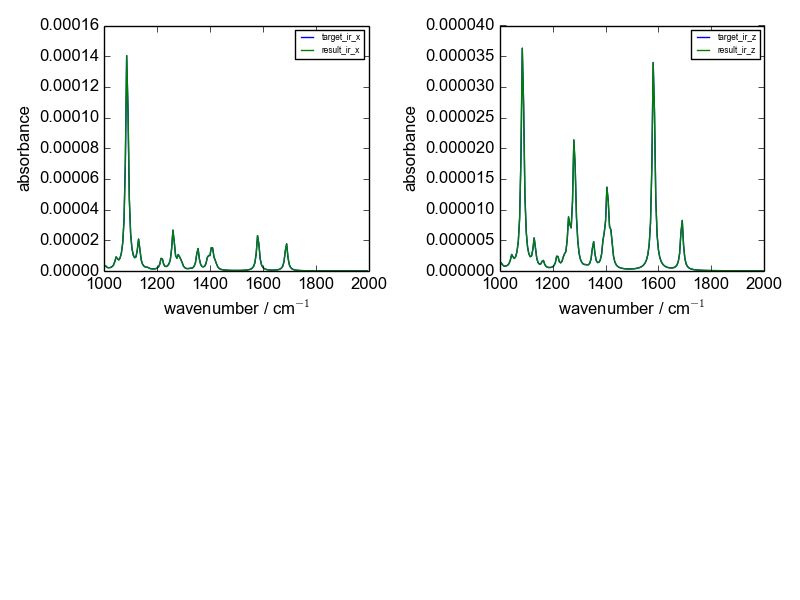
\includegraphics[scale=0.7]{Figures/ir_xz_result_plotting.png}
\caption{Compare target IR spectra with the ones generated by the return composition of Expreiment 1, 2 and 3}  \label{fig:4.1}
\end{figure}

In Experiment 4, the LP model that constructed from combining IR and Raman spectral information is sufficient to obtain the target composition. When the difference in $\theta$ degree for candidates decreases from $20^{\circ}$ to $10^{\circ}$. Checking if Raman and IR together is still sufficient enough to derive the target composition is desired. Therefore, the following experiments are conducted as shown in Table \ref{tab:4.2}. \\

\begin{table} \tiny 
\resizebox{\textwidth}{!}{
\begin{tabular}{| l | p{3cm} | l | l |}
\hline
\# Candidates & \multicolumn{2}{l|}{4} \\ \hline
Candidates & \multicolumn{2}{l|}{[0, 10, 20, 30]} \\ \hline
Target Composition & \multicolumn{2}{l|}{[0.1, 0.5, 0.4, 0]} \\ \hline
Experiment index & \# Data Points & Result Composition \\ \hline
5 & 200(irx) \newline 200(irz)& [0.752528, 0, 0, 0.247472]  \\ \hline
6 & 200(irx) \newline 200(irz) \newline 200(ramanxx)& [0.1, 0.5, 0.4, 0] \\ \hline
7 & 200(ramanxx) \newline 200(ramanxy) \newline 200(ramanxz)& [0.1, 0.5, 0.4, 0] \\ \hline
8 & 200(ramanxx) \newline 200(ramanxy) \newline 200(ramanzz)& [0.1, 0.5, 0.4, 0] \\ \hline
9 & 200(ramanxx) \newline 200(ramanxy) \newline 200(ramanxz) \newline 200(ramanzz)& [0.1, 0.5, 0.4, 0] \\ \hline
\end{tabular} 
%\end{center}
}
\caption{Experiment 5 to Experiment 9 setting for methionine candidates}
\label{tab:4.2}
\end{table}	

Experiment 5 shows that the LP model constructed by merely using IR spectral information is not sufficient to derive the target composition. Experiment 6 indicates that combining IR and Raman spectral information helps to derive the target composition. What's more, Experiment  7, 8 and 9, illustrate that Raman spectral information itself is sufficient to obtain the target composition as well. \\

For experiment setting in Table \ref{tab:4.1} and Table \ref{tab:4.2}, combining IR and Raman spectral information to construct a LP model is sufficient enough to obtain the target composition. In order to study the limitation of the LP model, the complexity of the experiment setting needed to be increased. Therefore, another group of experiments are designed as shown in Table \ref{tab:4.3}. There are 5 candidates included in the experiments. Each candidate has $\theta$ with the following degree: $0^{\circ}$, $10^{\circ}$, $20^{\circ}$, $30^{\circ}$ and $40^{\circ}$. The target composition is more complex than previous experiments, each candidate takes 20\% in the mixture. \\

Experiment 10 uses only IR spectral information to construct the LP model, and the return composition does not match the target one. Experiment 11 uses only Raman spectral information, and the return composition does not match to the target neither. Same for Experiment 12 that uses only SFG spectral information. From Experiment 13, different kinds of spectral information are combined. In Experiment 13, IR and Raman spectral information is used to produce the LP model, still the return composition is different from the target one. Experiment 14 combines Raman and SFG, Experiment 15 uses IR and SFG, Experiment 16 cooperates all the three spectral information, however, none of them returns a composition that matches the target one. \\

The results of Experiment 10 to 16 indicate that even combining all the spectral information of IR, Raman and SFG, it is still not sufficient to attain the target composition for the experiments set up in Table \ref{tab:4.3}. Our LP model is showing its limitation in these experiments. In order to confirm the reason causing the LP model to returning the target composition is because of insufficient information, further experiments are conducted in Table \ref{tab:4.4}. \\

\begin{table} \tiny
\begin{center}
\resizebox{\textwidth}{!}{
\begin{tabular}{| l | p{3cm} | l | l |}
\hline
Number of Candidates & \multicolumn{2}{l|}{5} \\ \hline
Candidates & \multicolumn{2}{l|}{[0, 10, 20, 30, 40]} \\ \hline
Target Composition & \multicolumn{2}{l|}{[0.2, 0.2, 0.2, 0.2, 0.2]} \\ \hline
Experiment index & Constraints & Result  \\ \hline
10 & 200(irx) \newline 200(irz)& [0.607766, 0, 0, 0, 0.392234]  \\ \hline
11 & 200(ramanxx) \newline 200(ramanxy) \newline 200(ramanxz) \newline 200(ramanzz)& [0.247792, 0, 0.502139, 0, 0.250069]  \\ \hline
12 & 200(sfgyyz) \newline 200(sfgyzy) \newline 200(sfgzzz)& [0.321014, 0, 0.31018, 0.163041, 0.205764]  \\ \hline
13 & 200(irx) \newline 200(irz) \newline 200(ramanxx) \newline 200(ramanxy) \newline 200(ramanxz) \newline 200(ramanzz)& [0.247792, 0, 0.502139, 0, 0.250069]  \\ \hline
14 & 200(ramanxx) \newline 200(ramanxy) \newline 200(ramanxz) \newline 200(ramanzz) \newline 200(sfgyyz) \newline 200(sfgyzy) \newline 200(sfgzzz)& [0.321014, 0, 0.31018, 0.163041, 0.205764]  \\ \hline
15 & 200(irx) \newline 200(irz) \newline 200(sfgyyz) \newline 200(sfgyzy) \newline 200(sfgzzz)& [0.321014, 0, 0.31018, 0.163041, 0.205764]  \\ \hline
16 & 200(irx) \newline 200(irz) \newline 200(ramanxx) \newline 200(ramanxy) \newline 200(ramanxz) \newline 200(ramanzz) \newline 200(sfgyyz) \newline 200(sfgyzy) \newline 200(sfgzzz)& [0.321014, 0, 0.31018, 0.163041, 0.205764]  \\ \hline
\end{tabular} 
}
\end{center}
\caption{Experiment 10 to Experiment 16 setting for methionine candidates} \label{tab:4.3}
\end{table}

\section{Experiments to Explain the Limitation of LP Model for Methionine Molecule}

In order to further explore the reason that LP model reaches its limitation for the real molecule, Experiment 17 and 18 are conducted. Methionine candidates are still used. To make the study case more general than Experiment 1 to 16, candidates' $\theta$ values are expanded from $0^{\circ}$ to $80^{\circ}$. In total, there are $9$ candidates. Because the SFG spectra for $\theta$ of $90^{\circ}$ is a straight line, it is excluded from all the experiments related to real molecules. For target composition, five candidates are randomly selected to be presented. The difference between Experiment 17 and 18 is that different amount of data points are selected to build the LP model. From all three spectroscopy techniques' spectral information, every 5 wavenumber a data point is selected for Experiment 17. Every 500 wavenumber a data point is selected for Experiment 18. As a result, Experiment 17 and 18 each returns a different composition. Both compositions do not match to the target one. \\

However, for both Experiment 17 and 18, when the return composition is used to generate the IR, Raman and SFG spectra, then these spectra are plotted together with the spectra created by the target composition. All the spectra are almost identical for IR, Raman and SFG. Figure \ref{fig:4.2}, \ref{fig:4.3} and \ref{fig:4.4} display the spectra plotted by using the return composition and the target one of Experiment 17. Every spectrum is almost identical to each other as shown in the figures. Same for Experiment 18 as shown in Figure \ref{fig:4.5}, \ref{fig:4.6} and \ref{fig:4.7}. These figures prove again that there are more than one composition that can perfectly construct the target spectra. The data information used to construct the LP model is not sufficient to converge to the return compostion exactly matches to the target one. This conclusion exactly fits the result obtained from the experiments we have done with the toy model.\\

\begin{table} 
\begin{center}
\resizebox{\textwidth}{!}{
\begin{tabular}{| l | p{3cm} | l | l }
\hline
\# Candidates & \multicolumn{2}{l|}{9} \\ \hline
Candidates & \multicolumn{2}{l|}{[0, 10, 20, 30, 40, 50, 60, 70, 80]} \\ \hline
Target Composition & \multicolumn{2}{l|}{[0.2201, 0.28905, 0.05201, 0.08251, 0.35633, 0, 0, 0, 0]} \\ \hline
Experiment \# & \# of Data Points & Result Composition \\ \hline
17 & each 5 wavenumber of IR, \newline Raman and SFG spectra & [0.158921, 0.388434, 0.0, 0.0985466, 0.354099, 0.0, 0.0, 0.0, 0.0] \\ \hline
18 & each 500 wavenumber of IR, \newline Raman and SFG spectra & [0.397991, 0.0, 0.203394, 0.0357663, 0.362848, 0.0, 0.0, 0.0, 0.0] \\ \hline
\end{tabular} 
}
\end{center}
\caption{Experiment 17 and 18 to explain the limitation of our LP model for methionine molecule}
\label{tab:4.4}
\end{table}	

\begin{figure}[!ht] 
\centering
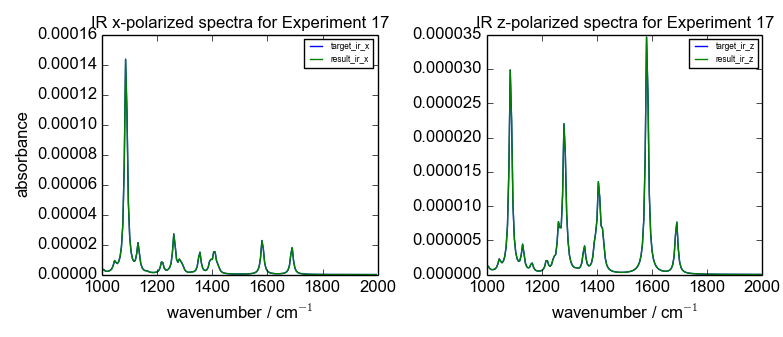
\includegraphics[scale=0.5]{Figures/chapter4_result_target_plotting_5datapoint_ir.png}
\caption{IR spectra plotted by using target composition and return composition of Experiment 17} \label{fig:4.2}
\end{figure}

\begin{figure}[!ht] 
\centering
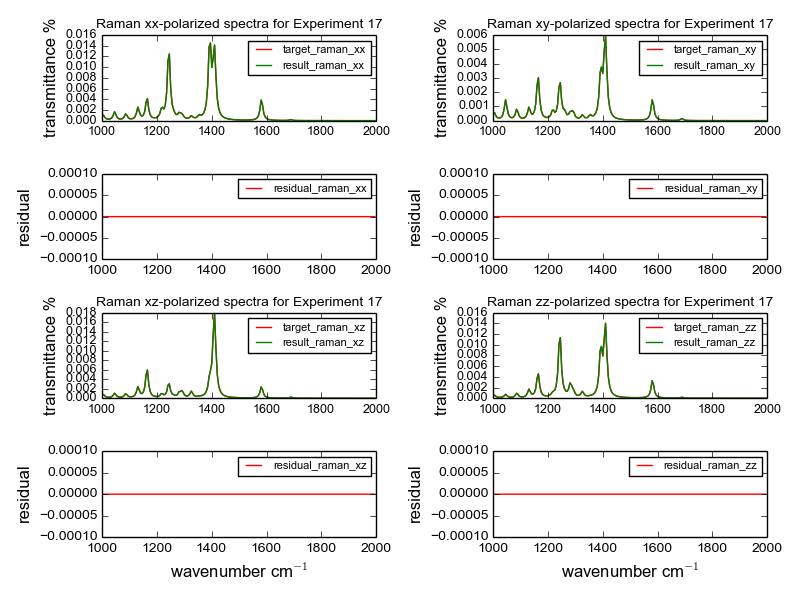
\includegraphics[scale=0.7]{Figures/chapter4_result_target_plotting_5datapoint_raman.png}
\caption{Raman spectra plotted by using the target composition and the return composition of Experiment 17} \label{fig:4.3}
\end{figure}

\begin{figure}[!ht]
\centering
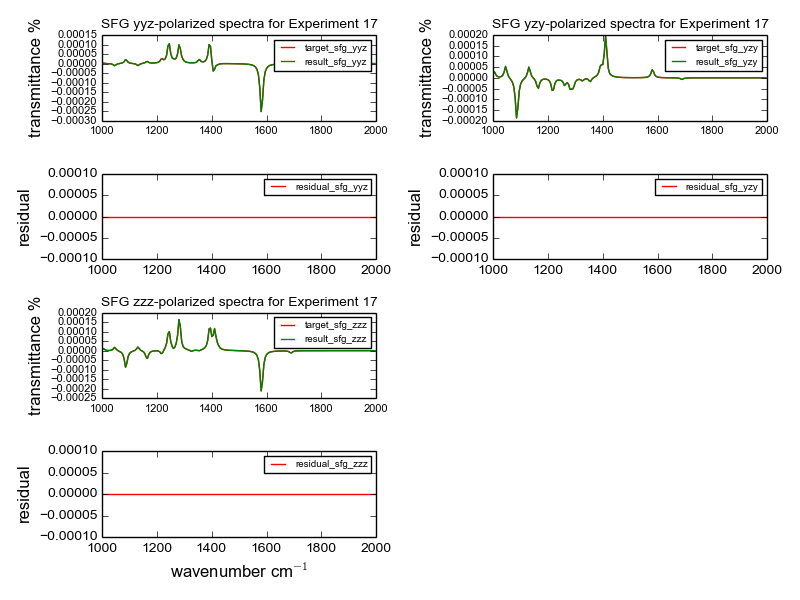
\includegraphics[scale=0.7]{Figures/chapter4_result_target_plotting_5datapoint_sfg.png}
\caption{SFG spectra plotted by using the target composition and the return composition of Experiment 17}  \label{fig:4.4}
\end{figure}

\begin{figure}[!ht] 
\centering
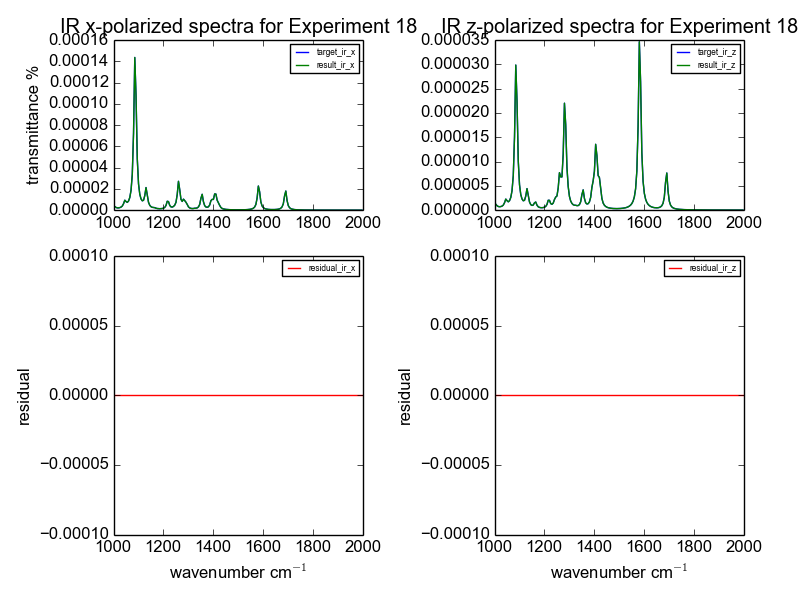
\includegraphics[scale=0.7]{Figures/chapter4_result_target_plotting_500datapoint_ir.png}
\caption{IR spectra plotted by using the target composition and the return composition of Experiment 18} \label{fig:4.5}
\end{figure}

\begin{figure}[!ht] 
\centering
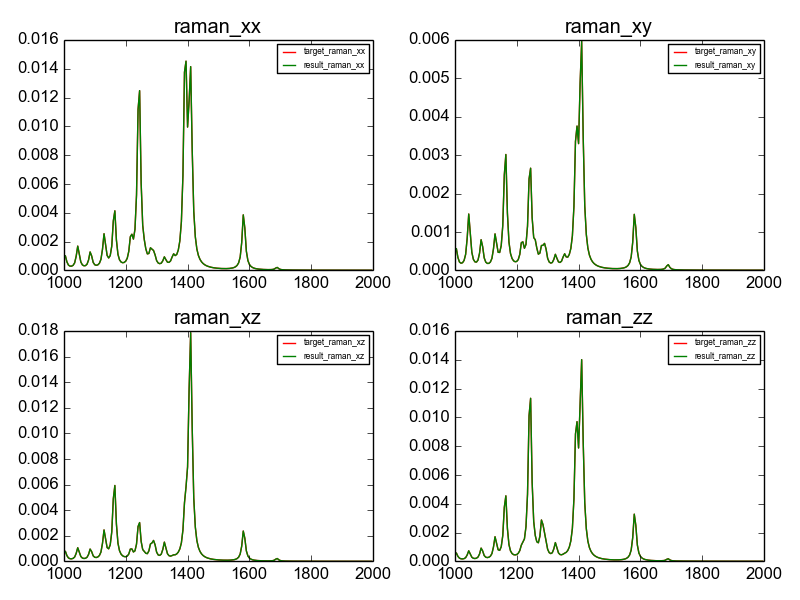
\includegraphics[scale=0.7]{Figures/chapter4_result_target_plotting_500datapoint_raman.png}
\caption{Raman spectra plotted by using the target composition and the return composition of Experiment 18} \label{fig:4.6}
\end{figure}

\begin{figure}[!ht] 
\centering
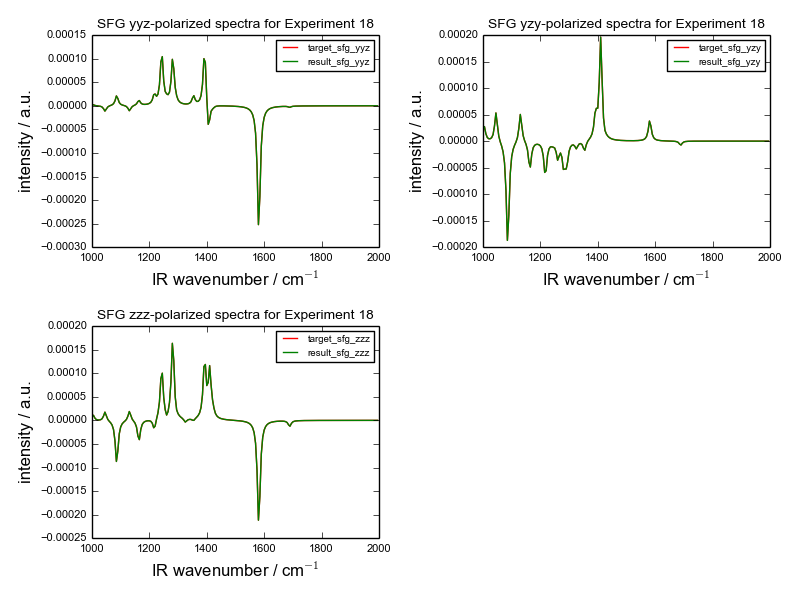
\includegraphics[scale=0.7]{Figures/chapter4_result_target_plotting_500datapoint_sfg.png}
\caption{SFG spectra plotted by using the target composition and the return composition of Experiment 18} \label{fig:4.7}
\end{figure} 

\section{Conclusion}

\section{Extra Experiments}
TODO: this part of experiments are similar as what are done in Chapter 5 and 6. Think how to involve this part properly.

From Experiment 1 to 18, LP model helps to return the target composition for some cases, and not for others. We want to figure out if there a clean line indicating the information used to generate the LP model is not sufficient to obtain the target composition for one molecule. In order to answer this question, more systematic experiments needed to be organized. Therefore, the following experiments are conducted. The Methionine candidate space is the same as Experiment 17 and 18. spread from $0^{\circ}$ to $80^{\circ}$ on $\theta$. 





